\documentclass{beamer}
\usetheme{Madrid}
\usecolortheme{whale}
\usepackage{amsmath,amssymb,amsfonts}
\usepackage{graphicx}
\usepackage{tikz}
\usetikzlibrary{arrows,shapes,positioning,fit}

\newcommand{\Loss}{\mathcal{L}}
\newcommand{\R}{\mathbb{R}}
\newcommand{\E}{\mathbb{E}}
\newcommand{\He}{\mathrm{He}}

\title{On a Mathematical Understanding of Loss of Plasticity}
\author{Presentation based on research paper}
\date{\today}

\begin{document}

\begin{frame}
    \titlepage
\end{frame}

\begin{frame}{Outline}
    \tableofcontents
\end{frame}

\section{Introduction}

\begin{frame}{}
    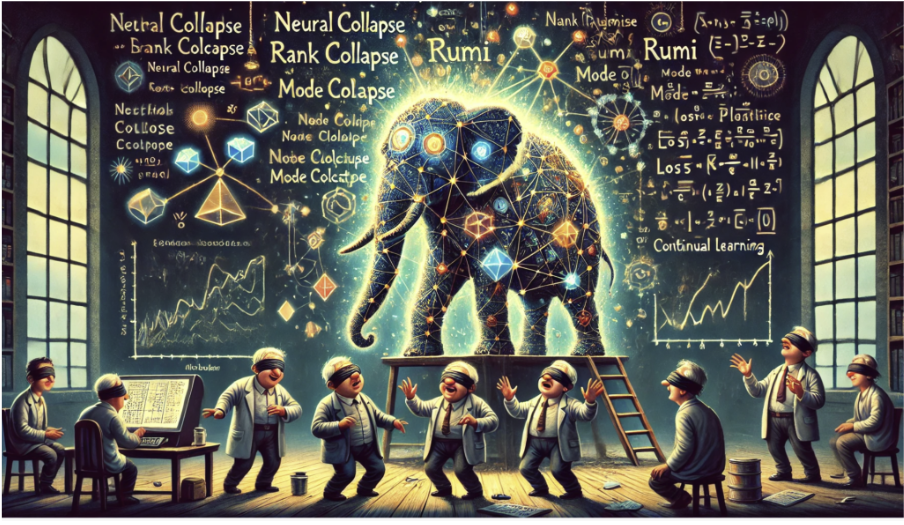
\includegraphics[width=\textwidth]{images/fun.png}
\end{frame}

\begin{frame}{The Problem of Loss of Plasticity}
    \begin{itemize}
        \item \textbf{Definition:} Neural networks may not adapt to new tasks after extended training, despite overparameterization
        \item \textbf{Richard Sutton's observations:}
        \begin{itemize}
            \item Large networks eventually learn no better than shallow models
            \item Weights grow in magnitude
            \item Neurons become ``dead'' or ``saturated''
            \item Internal representations lose diversity (drop in effective rank)
        \end{itemize}
        \item \textbf{Our goal:} Provide a mathematical foundation to understand how loss of plasticity:
        \begin{itemize}
            \item Formally define it
            \item Prove that it can theoretically happen
            \item Explore mitigation and recovery strategies
        \end{itemize}
    \end{itemize}
\end{frame}

\begin{frame}{}
    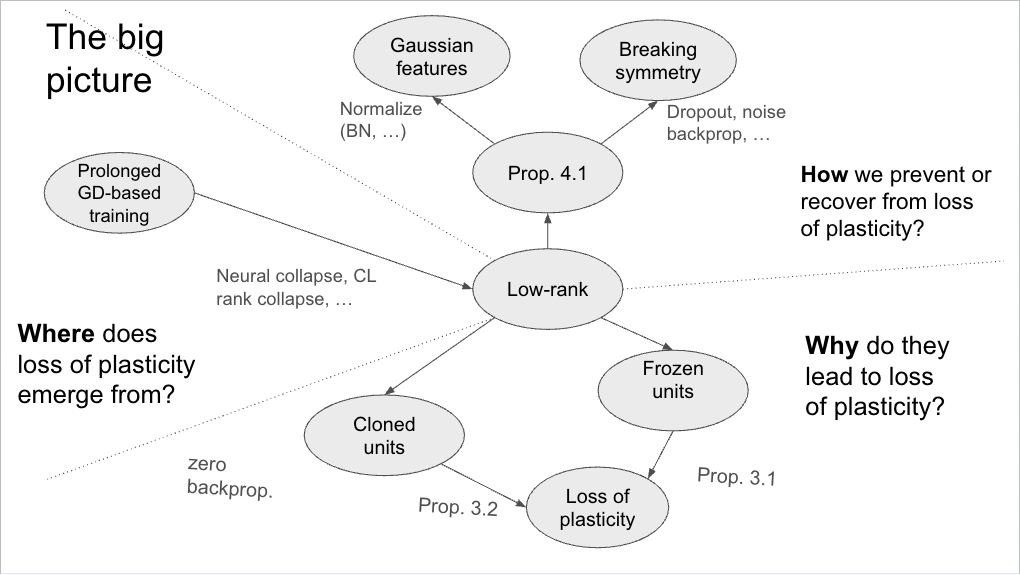
\includegraphics[width=\textwidth]{images/bp.png}
\end{frame}

\section{Mathematical Formalization}

\begin{frame}{Formal Definition of Loss of Plasticity}
    \begin{block}{Loss of Plasticity}
        Given a model with parameters $\theta$ and parameter space $\Theta$ with a manifold $\mathcal{M} \subseteq \Theta$ where:
        \begin{align}
            \forall \theta \in \mathcal{M} \implies \nabla_\theta\mathcal{L}(\theta) \in T_\theta\mathcal{M}
        \end{align}
    \end{block}
        \begin{block}{Manifold Stability}
        Based on Hessian properties in normal directions:
        \begin{align}
            &\text{Stable manifold:}\ \forall v \in N_\theta\mathcal{M} \setminus \{0\} \implies v^T\nabla_\theta^2 \mathcal{L}(\theta)v > 0 \\
            &\text{Unstable manifold:}\ \forall v \in N_\theta\mathcal{M} \setminus \{0\} \implies v^T\nabla_\theta^2 \mathcal{L}(\theta)v < 0
        \end{align}
    \end{block}
    
    \begin{itemize}
        \item Once model reaches manifold $\mathcal{M}$, it never escapes under gradient flow
        \item Parameter updates remain on lower-dimensional manifold
    \end{itemize}
\end{frame}

\section{Mechanisms of Loss of Plasticity}

\begin{frame}{Frozen Units:}
    \begin{block}{Proposition 3.1: Saturated Unit $\implies$ Frozen Upstream Parameters}
        If an activation $h_i(\cdot)$ that is always saturated on the training set $\frac{\partial h_i(x;\Theta)}{\partial z} = 0,$
        its upstream parameters $\theta \in \Theta_{\text{upstream}}$ remain frozen. 
        % \begin{align*}
        %     \frac{\partial \Loss}{\partial \theta} = 
        %     \frac{\partial \Loss}{\partial h_i} \cdot
        %     \underbrace{\frac{\partial h_i}{\partial z}}_{0} \cdot
        %     \frac{\partial z}{\partial \theta} = 0
        % \end{align*}
    \end{block}
    
    \begin{alertblock}{Common Sources of Saturation}
        \begin{itemize}
            \item Corresponds to a manifold $\mathcal{M}$ parallel to frozen axes. 
            \item Sigmoid/Tanh: Derivative $\approx 0$ for large inputs
            \item ReLU: "Dead ReLUs" with consistently negative inputs
            \item Softmax: Dominant logit suppresses gradients for others.
            % \item Attention: dominant attention weights freeze certain heads
        \end{itemize}
    \end{alertblock}
\end{frame}

\begin{frame}{Cloned Units Mechanism}
    \begin{columns}
        \begin{column}{0.5\textwidth}
            \begin{block}{Proposition 3.2: Weight Cloning Causes Loss of Plasticity}
                If a large network $\mathcal{G}$ has its nodes partitioned such that each partition behaves as a single node in a smaller network, such that incoming and outgoing weights are constant across partitions, it will always remain restricted to the smaller network, despite having more parameters.  
            \end{block}
            
            \begin{alertblock}{Key Insight}
                This is \textbf{structural loss of plasticity} - occurs regardless of data distribution. 
            \end{alertblock}
        \end{column}

        \begin{column}{0.5\textwidth}
            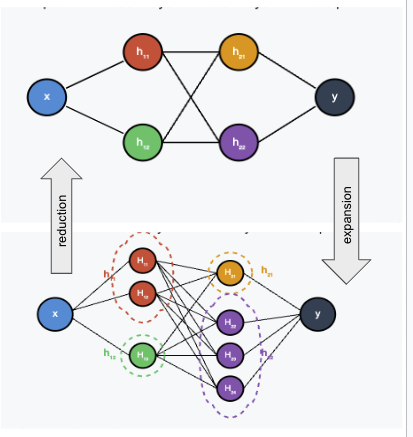
\includegraphics[width=\textwidth]{images/covering.png}
        \end{column}
    \end{columns}
\end{frame}

\begin{frame}{}
    \centering{
    \huge{Does this really happen?}\\
    \large{\href{https://ajoudaki.github.io/personal-notes/CL-demo.html}{demo: https://ajoudaki.github.io/personal-notes/CL-demo.html}
    }}
\end{frame}

\section{Prevention and Recovery}
\begin{frame}{}
    \centering{
    \huge{Can we mitigate or prevent this?}}
\end{frame}

\begin{frame}{Mitigating Loss of Plasticity}
    \begin{block}{Proposition 4.1: Rank Preservation}
        If activation function $f$ is: square-integrable with respect to Gaussian kernel, and not a bounded degree polynomial. And pre-activations are:
        \begin{itemize}
            \item Gaussian distributed: $x_i \sim \mathcal{N}(0,1)$
            \item Not duplicates: $\E[x_i x_j] = \rho_{ij}, |\rho_{ij}| < 1$
        \end{itemize}
        
        Then post-activation covariance $\E[f(x)^\top f(x)]$ is full rank
    \end{block}
    
    \begin{alertblock}{Practical Strategies}
        \begin{itemize}
            \item \textbf{Promote Gaussianity}: Use BatchNorm instead of LayerNorm
            \item \textbf{Explore stronger normalization}: Correct for higher-order statistics
            \item \textbf{Break symmetry}: Use dropout to prevent feature cloning
            \item \textbf{Parameter perturbation}: Escape manifold if Hessian has negative curvature
        \end{itemize}
    \end{alertblock}
\end{frame}





\begin{frame}{Recovery with perturbations: depends on curvature}
    Let $\theta_0 \in \mathcal{M}$ and consider a small perturbation in the normal direction $\epsilon v$, where $v \in N_{\theta_0}\mathcal{M}$ with $\|v\| = 1$ and $\epsilon > 0$ small. 
    
    Under gradient flow dynamics, the instantaneous rate of change of the squared distance to the manifold can be expressed as:
    \begin{align}
        \left.\frac{d}{dt}\right|_{t=0} \text{dist}^2(\theta_0 + \epsilon v, \mathcal{M}) = -2\epsilon \cdot v^T\nabla_{\theta}^2\mathcal{L}(\theta_0)v + O(\epsilon^2)
    \end{align}
We will have 
    \begin{itemize}
      \item $\text{Stable if } v^T\nabla_{\theta}^2\mathcal{L}(\theta_0)v > 0 \rightarrow \text{distance decreases} $
      \item $\text{Unstable if } v^T\nabla_{\theta}^2\mathcal{L}(\theta_0)v < 0 \rightarrow \text{distance increases} $
      \item $\text{Neutral if } v^T\nabla_{\theta}^2\mathcal{L}(\theta_0)v = 0 \rightarrow \text{higher-order terms decide} $
    \end{itemize}
    \begin{block}{}
              \item This is related to the noisy cloning! 
    \end{block}
\end{frame}

\begin{frame}{Empirically: The curvature of loss in continual learning }
    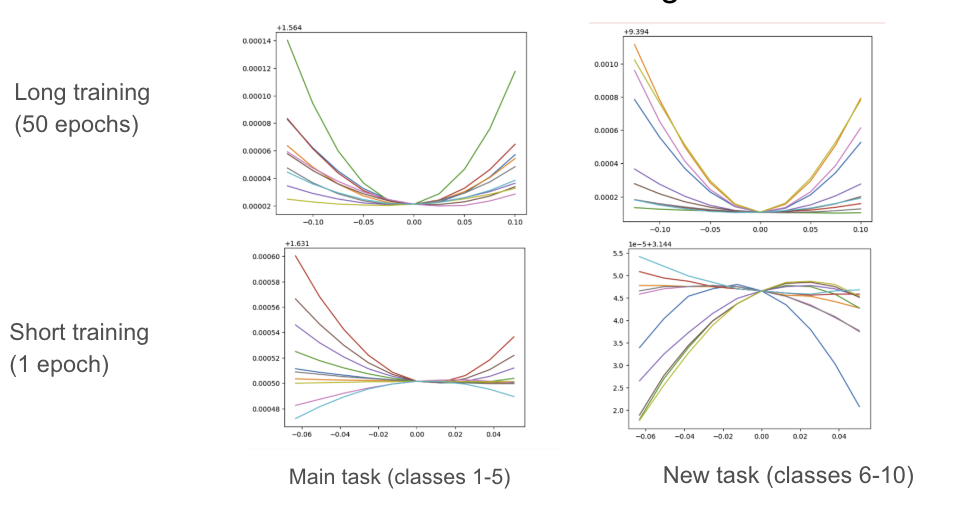
\includegraphics[width=\textwidth]{images/hess.png}
    Thus, this is task-dependent. Does it transfer between tasks? 
\end{frame}

\section{Conclusion}

\begin{frame}{Discussion and open questions}
    % \begin{block}{Summary}
    %     \begin{itemize}
    %         \item Formalized loss of plasticity as parameter trajectory restricted to a lower-dimensional manifold
    %         \item Identified two key mechanisms:
    %         \begin{itemize}
    %             \item Frozen units (saturation-based)
    %             \item Cloned units (duplication-based)
    %         \end{itemize}
    %         \item Both mechanisms create affine subspaces that trap gradient-based learning
    %     \end{itemize}
    % \end{block}
    
    \begin{alertblock}{Open Questions}
        \begin{itemize}
            \item How does the loss curvature look like in practice?
            \item Can we use BN in transformers?
            \item Can we use a stronger BN (higher order statistics)?
            \item Are there non-linear manifolds for loss of plasticity? 
        \end{itemize}
    \end{alertblock}
\end{frame}

\end{document}